\documentclass[UTF8]{ctexbeamer}
\usepackage{latexsym}
\usepackage{amsmath,amssymb}
\usepackage{color,xcolor}
\usepackage{graphicx}
\usepackage{algorithm}
\usepackage{amsthm}

\newtheorem{exercise}[theorem]{练习} %*去除编号

\usetheme{AnnArbor}
\usefonttheme[onlymath]{serif}
\usecolortheme{crane}

\title{数列极限与函数极限}
\subtitle{Week 1}

\author[chhzh123]{陈鸿峥}
\institute[]{\small\url{https://github.com/chhzh123/Notes-of-Math/blob/master/Mathematical_analysis/main.pdf}}
\date[Dec 1, 2018]{December, 2018}

\subject{Limit}
\keywords{}

\begin{document}

\begin{frame}
\titlepage
\end{frame}

\begin{frame}
\tableofcontents[subsectionstyle=show]
\end{frame}

\section{课程简介}
\begin{frame}
\sectionpage
\end{frame}

\begin{frame}{课程简介}
\begin{itemize}
	\item<1-> 不会重新将课本内容讲一遍
	\item<2-> 相关知识点的归纳整合,高于课本的观点
	\item<3-> 主要讲解题思路,例题均来自课本或考试真题
	\item<4-> 两周一次课,至多4次的样子
	\item<5-> 课件和笔记都可以在我的Github上找到
	\begin{center}
	\url{https://github.com/chhzh123/Notes-of-Math}
	\end{center}
	\item<6> 课程调查
\end{itemize}
\end{frame}

\section{课程安排}
\begin{frame}
\sectionpage
\end{frame}

\begin{frame}{课程安排}
大概是以下几个专题:
\begin{itemize}
	\item \textbf{数列极限与函数极限}\\
	对应课本第3章,笔记第2章
	\item \textbf{函数的一切}\\
	对应课本第2章、第3章第4节、第5章,笔记第3章、第4章
	\item \textbf{不定积分与定积分}\\
	对应课本第6章、第7章,笔记第5章、第6章
	\item \textbf{待定}
\end{itemize}
\end{frame}

\section{极限的概念}
\begin{frame}
\sectionpage
\end{frame}

\subsection{极限的定义}
\begin{frame}{极限的定义}
\begin{itemize}
	\item 数列极限 $\displaystyle\lim_{n\to\infty}x_n=A$
	\[\forall\varepsilon>0,\exists N\in\mathbb{Z}^+,s.t.\,n>N:|x_n-A|<\varepsilon\]
	\item 函数极限 $\displaystyle\lim_{x\to x_0}f(x)=A$
	\[\forall\varepsilon>0,\exists\delta>0,s.t.\,x\in\mathring{U}(x_0,\delta):|f(x)-A|<\varepsilon\]
\end{itemize}
\end{frame}

\begin{frame}{极限的定义}
\begin{figure}
\centering
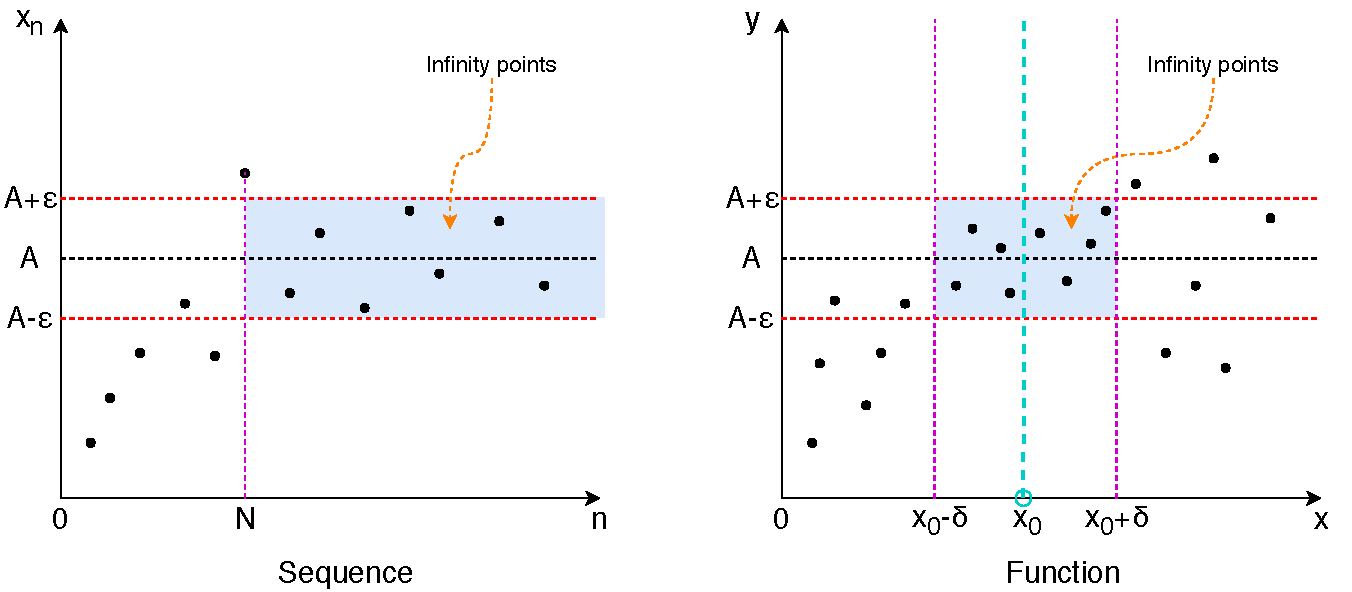
\includegraphics[width=\linewidth]{fig/Limit_def.pdf}
\end{figure}
\end{frame}

\subsection{极限的几个重要性质}
\begin{frame}{极限的几个重要性质}
对于数列极限和函数极限都有:
\begin{enumerate}
	\item<1-> (局部)有界性:有极限必有界 $\to$ 单调有界原理
	\item<2-> \textbf{(局部)保号性}:必存在与极限同号的值
	\item<3-> (局部)保序性:极限序关系成立,原式序关系也成立
	\item<4-> 唯一性:极限存在必唯一
	\item<5-> 夹迫性:夹逼定理
	\item<6-> 极限不等式:原式序关系成立,极限序关系成立
\end{enumerate}
\end{frame}

\subsection{沟通两种极限的桥梁}
\begin{frame}{沟通两种极限的桥梁}
\begin{theorem}[海涅定理]
\[\lim_{x\to x_0}f(x)=A\]
等价于\[\forall\{x_n\},\lim_{n\to\infty}x_n=x_0,x_n\ne x_0(n=1,2,\cdots)\;:\lim_{n\to \infty}f(x_n)=A\]
\end{theorem}
注:常用来证明函数极限不存在或作逼近用
\begin{example}[\textsection 3.3/11]
\[\lim_{x\to 0}\cos\frac{1}{x}\]
\end{example}
\end{frame}

\begin{frame}{补充习题:海涅定理}
\begin{exercise}[\textsection 3.3/12]
证明$\lim_{x\to x_0}D(x)$不存在,其中
\[D(x)=\begin{cases}1&x\in\mathbb{Q}\\0&x\notin\mathbb{Q}\end{cases}\]
\end{exercise}
Tips: 分为有理数和无理数讨论,并将无理数小数形式设出来\\
其他习题:\textsection 3.3/8,18
\end{frame}


\section{极限的证明与计算}
\begin{frame}
\sectionpage
\end{frame}

\subsection{常见的极限计算方法}
\begin{frame}
\subsectionpage
\end{frame}

\begin{frame}{1. 直接代入}
即极限的四则运算,一定要\textcolor{red}{先对极限式化简(分子/分母有理化、因式分解)},然后将趋于极限的值代入看是否是\textbf{未定型},若不是则可直接得到答案
% 化简对于求任意极限都很重要
\begin{example}[\textsection 3.3/2(5)]
\[\lim_{x\to 3}\frac{\sqrt{1+x}-2}{x-3}\]
\end{example}
\begin{example}[17数分期中]
\[\lim_{x\to 1}\left(\frac{1}{1-x}-\frac{1}{x^2+x+1}\right)\]
\end{example}
% 不可直接判断,无穷减无穷可能是有限值
\end{frame}
% 四则运算的要小心

\begin{frame}{补充习题:直接代入}
\begin{exercise}[\textsection 3.2/7(2)]
% 除以最高次项
\[\lim_{n\to\infty}\frac{(-2)^n+3^n}{(-2)^{n+1}+3^{n+1}}\]
\end{exercise}
其他习题:\textsection 3.2/7(1)(4),\textsection 3.3/2,6
\end{frame}

\begin{frame}{补充习题:化简(求和积)}
\begin{exercise}[\textsection 3.3/13]
\[\lim_{n\to\infty}\cos\frac{x}{2}\cos\frac{x}{4}\cdots\cos\frac{x}{2^n}\]
\end{exercise}
\begin{exercise}[\textsection 3.2/8(7)]
\[\lim_{n\to\infty}(\sqrt{2}\sqrt[4]{2}\cdots\sqrt[2^n]{2})\]
\end{exercise}
其他习题:\textsection 3.2/8(1)(4),\textsection 3.3/13
\end{frame}

\begin{frame}{2. 化归重要极限}
\[\displaystyle\lim_{x\to 0}\frac{\sin x}{x}=1\qquad\qquad\lim_{x\to\infty}\left(1+\frac{1}{x}\right)^x=\lim_{x\to 0}(1+x)^{\frac{1}{x}}=\mathrm{e}\]
关注形式,重点在于\textbf{配凑}
\begin{example}[\textsection 3.3/10(9)]
\[\lim_{x\to 0}\frac{\sqrt{1-\cos x^2}}{1-\cos x}\]
\end{example}
\begin{example}[17数分期中]
\[\lim_{x\to 0}(1+\sin x)^{\frac{1}{2x}}\]
\end{example}
\end{frame}

\begin{frame}{补充习题:化归重要极限}
\begin{exercise}[\textsection 3.3/10(20)]
\[\lim_{x\to 0}\left(\frac{1+x}{1-x}\right)^{\frac{1}{x}}\]
\end{exercise}
其他习题:\textsection 3.3/10
\end{frame}

\begin{frame}{3. 洛必达}
\begin{itemize}
	\item 一定要先判断是否为\textcolor{red}{\Large 未定型}!
	\item 最没有技术含量的求极限,暴算就好了
	\item 求导后极限不存在不能说原极限不存在
	\item 一些奇怪的东西只要符合未定型也是可以用洛必达的
\end{itemize}
\begin{example}[\textsection 5.2/3]
设$f(x)$二阶可导,求证:
\[\lim_{h\to 0}\frac{f(x+2h)-2f(x+h)+f(x)}{h^2}=f''(x)\]
\end{example}
其他习题:\textsection 5.2/1
\end{frame}

\begin{frame}{4.1 夹逼(取两头)}
取两头,全部换成同一项,或者就只剩下一项
\begin{example}[17复旦高数]
\[\lim_{n\to\infty}\frac{1}{\sqrt{n^2}}+\frac{1}{\sqrt{n^2}+1}+\cdots+\frac{1}{\sqrt{(n+1)^2}}\]
\end{example}
\begin{example}[17数分期中]
\[\lim_{n\to\infty}\sqrt[n]{\cos^2 1+\cos^2 2+\cdots+\cos^2 n}\]
\end{example}
\end{frame}

\begin{frame}{4.2 夹逼(不等式放缩)}
均值不等式:
\[\frac{2}{\frac{1}{a}+\frac{1}{b}}\leq\sqrt{ab}\leq\frac{a+b}{2}\leq\sqrt{\frac{a^2+b^2}{2}}\]
配凑形式+消元
\begin{example}[\textsection 3.2/8(9)]
\[\lim_{n\to\infty}\frac{1}{2}\cdot\frac{3}{4}\cdot\cdots\cdot\frac{2n-1}{2n}\]
\end{example}
\end{frame}

\begin{frame}{补充习题:夹逼}
\begin{exercise}[\textsection 3.2/11]
设$a_1,a_2,\ldots,a_m$为$m$个正数,证明:
\[\lim_{n\to\infty}\sqrt[n]{a_1^n+a_2^n+\cdots+a_m^n}=\max(a_1,a_2,\ldots,a_m)\]
\end{exercise}
\begin{exercise}[\textsection 3.2/8(10)]
\[\lim_{n\to\infty}\sqrt[n]{\frac{1}{2}\cdot\frac{3}{4}\cdot\cdots\cdot\frac{2n-1}{2n}}\]
\end{exercise}
其他习题:\textsection 3.2/8(2)(3)(5)(12)
\end{frame}

\begin{frame}{5. 无穷小量替换}
实际上是一阶泰勒公式,有适用范围:一般极限乘除才可用
\begin{itemize}
	\item $\arcsin x\thicksim\sin x\thicksim x$
	\item $\arctan x\thicksim\tan x\thicksim x$
	\item $\ln(1+x)\thicksim x$
	\item $\displaystyle \cos x\thicksim 1-\frac{x^2}{2}$
	\item $e^x\thicksim 1+x$
	\item $\displaystyle \sqrt[n]{1+x}-1\thicksim\frac{x}{n}$
\end{itemize}
\begin{example}
\[\lim_{x\to 0}\frac{1-\cos\sin x}{2\ln(1+x^2)}\] %-1/12
\end{example}
\end{frame}

\begin{frame}{补充习题:无穷小量替换}
\begin{exercise}[17数分期末]
\[\lim_{x\to 0}\frac{\sqrt{1+\sin x}-\sqrt{1+x}}{\sin^3 x}\]
\end{exercise}
\begin{exercise}[17数分期末]
\[\lim_{n\to\infty}n^2\left(\arcsin\frac{\pi}{4n}-\arcsin\frac{\pi}{4n+1}\right)\]
\end{exercise}
其他习题:\textsection 3.5/6
\end{frame}

\begin{frame}{6.1 其他方法(无穷小量乘有界量)}
无穷小量乘有界量极限值为$0$,常见于三角函数\\
(要熟悉三角和差化积、积化和差公式)
\begin{example}[17数分期中]
\[\lim_{x\to\infty}(\sin\sqrt{x+1}-\sin\sqrt{x})\]
\end{example}
\begin{exercise}[0x高数]
\[\lim_{n\to\infty}\frac{n^\frac{2}{3}\sin n^2}{n+1}\]
\end{exercise}
\end{frame}

\begin{frame}{6.2 其他方法(升指数)}
对幂函数取对数后取指数
\[\lim_{x\to x_0} f(x)^{g(x)}=\lim_{x\to x_0} \mathrm{e}^{\ln f(x)^{g(x)}}=\mathrm{e}^{\lim_{x\to x_0} g(x)\ln f(x)}\]
\begin{example}[\textsection 3.2例13]
\[\lim_{n\to\infty}\sqrt[n]{n}\]
\end{example}
\end{frame}

\begin{frame}{ 6.3 其他方法(分式递推)}
先证明单调(数学归纳法)有界,后利用单调有界定理证明极限存在,将极限值设出来,代入解方程
\begin{example}[\textsection 3.2/13(4)]
\[x_0=1,x_n=1+\frac{x_{n-1}}{1+x_{n-1}}\text{,求}\lim_{n\to\infty}x_n\]
\end{example}
其他习题:\textsection 3.2/13
\end{frame}

\subsection{用定义证明极限}
\begin{frame}
\subsectionpage
\end{frame}

\begin{frame}{1. 几种基本类型}
\begin{enumerate}
	\item 幂函数:$\displaystyle\frac{x^m}{x^n}(x\to\infty)=\frac{1}{x^{n-m}}\to 0$
	\item 幂指型:$\displaystyle\frac{x^k}{a^x}(a>1,x\to\infty)=\frac{x^k}{(1+b)^x}<\frac{x^k}{C_x^{k+1}x^{k+1}}\to 0$
	\item 指阶型:$\displaystyle\frac{a^n}{n!}(n\to\infty)=\frac{a}{n}\underbrace{\frac{a}{n-1}\cdots\frac{a}{a+1}}_{<1}\frac{a^a}{a!}<\frac{a}{n}\frac{a^n}{a!}\to 0$
	\item 阶炸型:$\displaystyle\frac{n!}{n^n}(n\to\infty)=\frac{n}{n}\underbrace{\frac{n-1}{n}\cdots\frac{2}{n}}_{<1}\frac{1}{n}<\frac{1}{n}\to 0$
\end{enumerate}
\end{frame}

\begin{frame}{2. 常见放缩}
\begin{enumerate}
	\item $x^a(a>0)<a^x(a>1)<x!$
	\item $\displaystyle n<\left(\frac{n}{2}\right)^{\frac{n}{2}}<n!<n^n\qquad$取对数可证
	\item $\displaystyle \frac{x}{x+1}\leq\ln(x+1)\leq x$
	\item $\displaystyle (1+x)^n>1+nx\qquad$伯努利(Bernoulli)不等式
	\item $\Big||a|-|b|\Big|\leq|a\pm b|\leq|a|+|b|\quad$\textbf{绝对值三角不等式}
	\item $\displaystyle \frac{2}{\frac{1}{a}+\frac{1}{b}}\leq\sqrt{ab}\leq\frac{a+b}{2}\leq\sqrt{\frac{a^2+b^2}{2}}\quad$\textbf{均值不等式}
	\item $[x]\leq x<[x]+1\qquad$高斯函数性质
\end{enumerate}
其他习题:\textsection 3.2/1,2,12(1),\textsection 3.3/1
\end{frame}

\begin{frame}{3. 有界量直接取界}
$\sin x,(-1)^n$等均直接取$\pm 1$
\begin{example}[\textsection 3.2/1(2)]
用定义证明
\[\lim_{n\to\infty}\frac{\sin n}{n}\]
\end{example}
\begin{example}[\textsection 3.2/1(4)]
用定义证明
\[\lim_{n\to\infty}\frac{n+(-1)^n}{n^2-1}\]
\end{example}
\end{frame}

\begin{frame}{4. 配凑+绝对值三角不等式}
在证明题中非常非常非常常见,之后各种关于极限的证明(包括微分积分)也都会用到,常常通过加一项减一项实现,关键在于\textbf{将结论往条件靠}!
\begin{example}[\textsection 3.2/16]
设$\displaystyle\lim_{n\to\infty}a_n=a$,证明
\[\lim_{n\to\infty}\frac{a_1+a_2+\cdots+a_n}{n}=a\]
\end{example}
\end{frame}

\begin{frame}{补充习题:配凑绝对值三角}
\begin{exercise}[\textsection 3.3/4]
设$f(x)>0$,证明:
\[\lim_{x\to x_0}f(x)=A\implies\lim_{x\to x_0}|f(x)|=|A|\]
\end{exercise}
其他习题:\textsection 3.2/3(2),6
\end{frame}

\subsection{总结}
\begin{frame}{极限计算方法 -- 总结}
\begin{enumerate}
	\item<1-> 不要着急一上来就洛必达,先试下简单方法是否可行
	\item<2-> 注意四则运算只能对\textbf{有限项}且\textbf{项数固定}的数列使用
	\item<3-> \textcolor{red}{\textbf{化简}}很重要,化简的形式也有很多种(除了有理化和因式分解,还有先求和求积等)
	\item<4-> 用定义证明数列极限放缩即可,注意不要变负;函数极限通常要先限制变量范围,如令$0<|x-x_0|<1$
	\item<5-> 计算题来来去去都是那几种方法,证明题也一定是\textbf{放缩配凑绝对值}
\end{enumerate}
\end{frame}

\end{document}